\chapter{\IfLanguageName{dutch}{Stand van zaken}{State of the art}}%
\label{ch:stand-van-zaken}

% Tip: Begin elk hoofdstuk met een paragraaf inleiding die beschrijft hoe
% dit hoofdstuk past binnen het geheel van de bachelorproef. Geef in het
% bijzonder aan wat de link is met het vorige en volgende hoofdstuk.

% Pas na deze inleidende paragraaf komt de eerste sectiehoofding.

\section{Keuze van het Model: Overwegingen en Argumentatie}
Bij het ontwikkelen van een model voor de automatische vertaling van Vlaamse Gebarentaal naar tekst is de keuze van het juiste model cruciaal. 
Verschillende factoren, zoals nauwkeurigheid, rekenkracht, trainingsvereisten en generaliseerbaarheid, spelen een rol in deze beslissing. 
In deze sectie wordt besproken welke modellen in overweging zijn genomen, welke evaluatiecriteria zijn gehanteerd en waarom het uiteindelijke model als de beste keuze werd beschouwd.
\\
\\
\subsection{Type modellen}
In gebarentaalherkenning heb je twee types van herkenning.\autocite{Ahn_Jang_Chung_Korea_Advanced_Institute_of_Science_and_Technology_2023}
\begin{enumerate}
  \item ISLR -> Isolated Sign Language Recognition
  \item CSLR -> Continouis Sign Language Recognition
\end{enumerate}
In dit onderzoek is er gekozen voor de tweede optie namelijk CSLR.
De keuze voor CSLR is gebaseerd op verschillende overwegingen. 
Allereerst komt continue gebarentaalherkenning veel beter overeen met de natuurlijke wijze waarop gebaren in de dagelijkse communicatie worden uitgevoerd. 
In tegenstelling tot ISLR, waarbij gebaren als afzonderlijke en duidelijk gesegmenteerde eenheden worden herkend, maakt CSLR het mogelijk om de vloeiende en dynamische overgang tussen opeenvolgende gebaren te analyseren. 
Dit zorgt voor een realistischer en natuurlijker vertaalproces, essentieel voor toepassingen in real-time communicatie.
\\
\\

Tot slot sluit de keuze voor CSLR beter aan bij de beoogde reële toepassingen. 
Gebruikers verwachten immers een vloeiende en natuurlijke interactie, waarin gebaren niet geïsoleerd maar in een doorlopende context worden gepresenteerd. 
Hoewel de implementatie en training van een CSLR-systeem complexer zijn, biedt het op de lange termijn een robuustere en gebruiksvriendelijkere oplossing voor automatische vertaling van gebarentaal.
\\
\\

Samenvattend ondersteunt de keuze voor CSLR de doelstelling van dit onderzoek: het ontwikkelen van een model dat niet alleen nauwkeurig gebaren kan herkennen, maar ook de dynamiek en continuïteit van natuurlijke gebarentaal effectief weet te verwerken.

\subsection{Mogelijke Modellen}
Er zijn veel mogelijke modellen die gebruikt kunnen worden in dit onderzoek. 
In dit gedeelde wordt allereerst een overzicht gegeven van de meest veelbelovende benaderingen, waarbij zowel traditionele als moderne deep learning methoden aan bod komen.
\\
\\
Een eerste optie is het gebruik van convolutionele neurale netwerken (CNN) voor het extraheren van visuele features uit videobeelden van gebaren. 
CNN's zijn zeer effectief in het herkennen van spatiale patronen en vormen vaak de basis voor modellen die visuele data verwerken\autocite{farahat2022novelfeaturescramblingapproachreveals}. 
Deze netwerken kunnen worden gecombineerd met sequentiemodellen, zoals Long Short-Term Memory (LSTM) of Gated Recurrent Units (GRU), om de temporele dynamiek van continue gebarentaal te modelleren\autocite{electronics13071229}.
\\
\\
Een tweede benadering betreft het gebruik van Transformer-gebaseerde modellen. 
Deze modellen, die hun oorsprong vinden in de natuurlijke taalverwerking, maken gebruik van self-attention mechanismen om lange-afstandsrelaties binnen sequenties vast te leggen. 
Dit is bijzonder waardevol voor de analyse van de continue stroom van gebaren, omdat het model zo beter contextuele informatie kan benutten \autocite{vaswani2023attentionneed}, \autocite{DU2022115}.
\\
\\
Daarnaast worden hybride modellen overwogen, waarbij bijvoorbeeld CNN's worden ingezet voor feature extractie en Transformers of RNN's voor de sequentiële interpretatie. 
Deze combinatie biedt het voordeel van een efficiënte verwerking van visuele data, terwijl de temporele samenhang binnen de gebarensequenties adequaat wordt gemodelleerd.
Hiervan zijn al meerdere voorbeelden zoals in de studie van \textcite{Wang2022}
\\
\\
Er bestaan veel opties in bovenstaande gebieden. 
Echter, een volledige implementatie waarbij een model van de grond af aan wordt opgebouwd en getraind, valt buiten de scope van dit onderzoek. 
Daarom wordt gekozen voor een aanpak die gebruikmaakt van bestaande, pre-getrainde modellen. 
Deze strategie stelt ons in staat de bewezen efficiëntie van gevestigde architecturen te benutten, terwijl we ons richten op de afstemming van deze modellen op de specifieke eisen van gebarentaalherkenning.
\\
\\
Het model dat hieruit is voortgekomen is het SlowFast Sign-model. 
Dit model is ontworpen voor de effectieve extractie van zowel statische als dynamische kenmerken uit videobeelden, een essentieel aspect voor Continuous Sign Language Recognition (CSLR). 
Hieronder volgt een nadere toelichting op de belangrijkste componenten van dit model, gebaseerd op de bevindingen in de literatuur:

\subsubsection{De kern van deze aanpak bestaat uit twee parallelle paden:}
\paragraph{De Slow Pathway:}
Deze pathway verwerkt de video-input met een lagere frame rate. 
Hierdoor legt het een stabiele en gedetailleerde representatie vast van ruimtelijke kenmerken, zoals handvormen, gezichtsuitdrukkingen en andere visuele details. 
Door gebruik te maken van een grotere temporele stride (bijvoorbeeld $\alpha$ = 4) wordt efficiënte verwerking van lange videosequenties mogelijk, zoals die vaak voorkomen in CSLR-datasets.
(Zie aflbeelding \ref{fig:structuur_slowFast})

\paragraph{De Fast Pathway:}
De fast pathway werkt met een hogere frame rate en richt zich op het vastleggen van de dynamische aspecten, zoals snelle armbewegingen en andere temporele veranderingen. 
Door de channelcapaciteit van deze pathway bewust lager te houden (bijvoorbeeld $\beta$ = 1/8 van de slow pathway) kan het model zich optimaal concentreren op het modelleren van de bewegingsdynamiek zonder teveel rekenkracht te verbruiken.
(Zie aflbeelding \ref{fig:structuur_slowFast})

\subsubsection{Feature Fusion Methoden}
Om de complementaire informatie van beide pathways optimaal te benutten, introduceert het model twee innovatieve fusion methoden:
\paragraph{Bi-directional Feature Fusion (BFF):}
BFF faciliteert de uitwisseling van informatie tussen de slow en fast pathways. 
In plaats van traditionele concatenatie, wordt hier een additionele operatiestrategie gebruikt. 
Hierbij worden de features eerst geprojecteerd via 3D-convoluties en vervolgens via een learnable parameter (initieel op 0 gezet) toegevoegd. 
Dit maakt een dynamische en kosteneffectieve integratie van zowel statische als dynamische semantiek mogelijk \autocite{10445841}.
\paragraph{Pathway Feature Enhancement (PFE):}
Deze methode introduceert extra sequentiemodules (auxiliary subnetwerken) om de verkregen representaties verder te verrijken. 
PFE versterkt zowel de spatial als de dynamic features, zonder dat er extra inference-tijd nodig is. 
Dit zorgt voor een verbeterde temporale alignering en een robuustere feature-representatie \autocite{10445841}.
\\
\\
\begin{figure}[h!]
  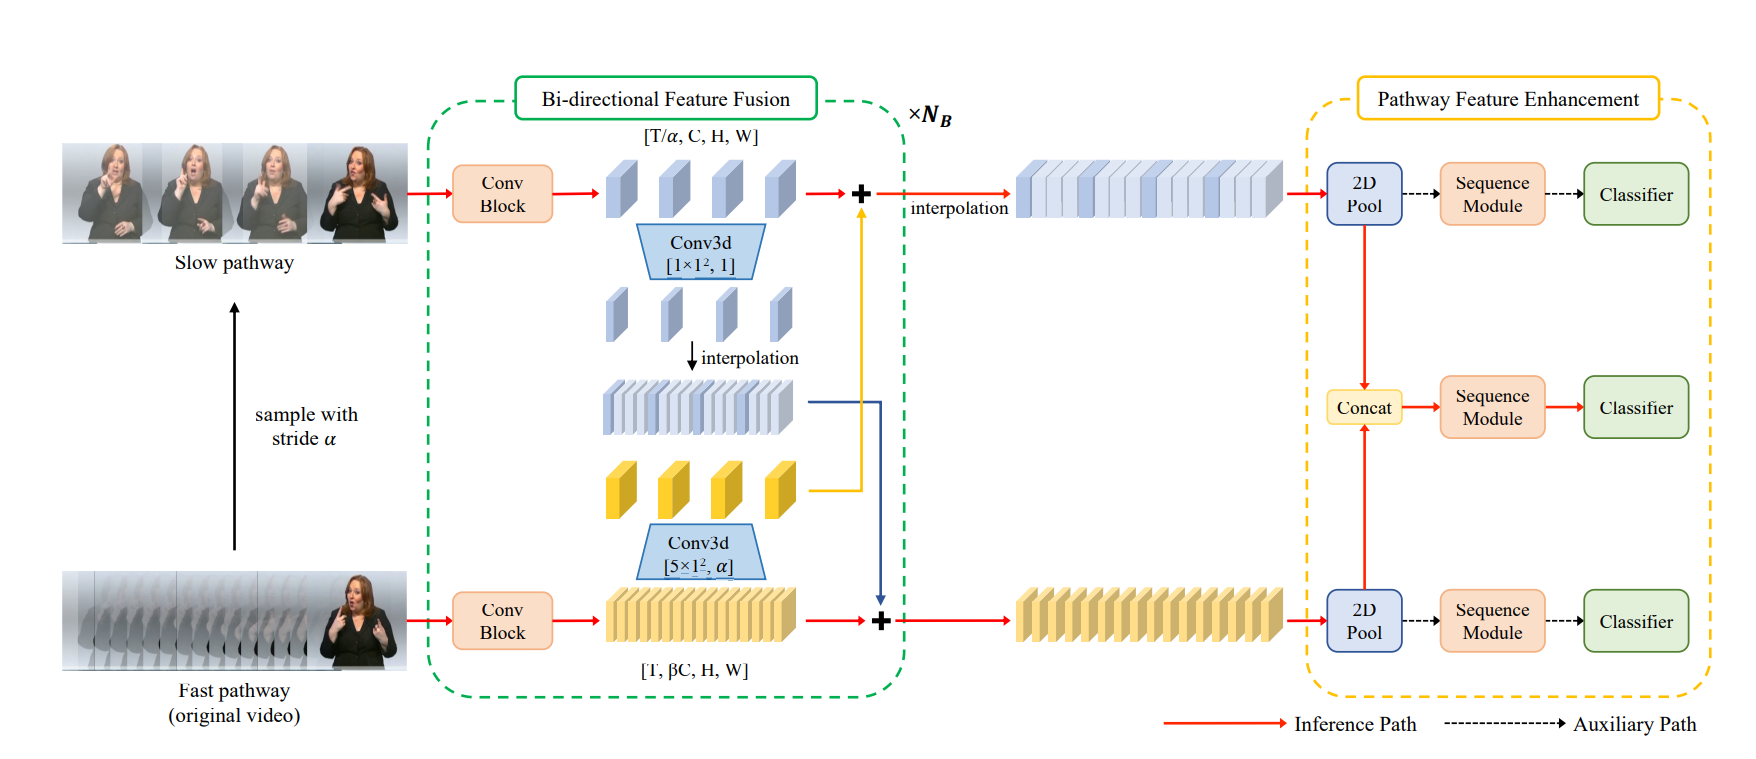
\includegraphics[width=0.5\textwidth]{../graphics/structuurSlowFast.png}
  \caption{Structuur van het Slow Fast Sign Model \autocite{10445841}.}
  \label{fig:structuur_slowFast}
\end{figure}

Voor het decoderen van de gebarensequenties maakt het SlowFast Sign-model gebruik van beam search. 
In plaats van per tijdstap slechts de meest waarschijnlijke voorspelling te kiezen, bewaart beam search meerdere mogelijke interpretaties (beam width $k$). 
Hierdoor kan het model niet alleen de meest waarschijnlijke gebaren herkennen, maar ook contextuele en grammaticale correctheid behouden. 
Dit zorgt voor robuustere en nauwkeurigere transcripten, vooral in situaties met ruis of ambiguïteit\autocite{10445841}.

\section{Overwegingen bij het Deployen van het Model}
Bij het implementeren van het model voor real-time vertaling van Vlaamse Gebarentaal naar tekst is de keuze van het platform een cruciale factor. 
Twee veelvoorkomende opties zijn een Android-app of een webgebaseerde oplossing. Beide benaderingen hebben hun eigen voordelen en uitdagingen op het gebied van prestaties, toegankelijkheid, gebruikservaring en rekenkracht. 
In deze sectie worden de voor- en nadelen van beide opties besproken, evenals de argumentatie achter de uiteindelijke keuze voor de deploymentstrategie.
\\
\\
Een model kan op twee manieren worden ingezet voor gebruik in een mobiele applicatie: On-device deployment (zie \ref{subsec:on-device}) en Cloud-based deployment (zie \ref{subsec:cloud-based}).
De keuze tussen deze methoden hangt af van factoren zoals real-time prestatie-eisen, energieverbruik, privacy en de technische mogelijkheden van de doelgroep.
\subsection{On-device}
\label{subsec:on-device}
Bij on-device deployment wordt het model lokaal uitgevoerd op het mobiele apparaat van de gebruiker. 
Dit heeft als voordeel dat er geen constante internetverbinding nodig is, wat zorgt voor een lagere latentie en betere privacybescherming. 
Daarnaast kan het model ook offline functioneren, wat cruciaal is voor gebruikers in gebieden met beperkte connectiviteit. 
Echter, on-device inferentie kan intensief zijn op het gebied van rekenkracht en batterijverbruik, zeker bij complexe deep learning-modellen. 
Volgens \textcite{8360327} vereist on-device inferentie vaak optimalisaties zoals modelcompressie of hardwareversnelling met behulp van TensorFlow Lite, ONNX Runtime of Core ML.

\subsection{Cloud-based}
\label{subsec:cloud-based}
Bij cloud-based deployment wordt het model niet op het mobiele apparaat zelf uitgevoerd, maar op een externe server. 
Dit heeft als voordeel dat krachtigere hardware gebruikt kan worden, wat leidt tot snellere inferentie en ondersteuning voor grotere modellen. 
Daarnaast maakt dit het gemakkelijker om updates door te voeren zonder dat de gebruiker iets hoeft te downloaden. 
Het nadeel is echter de afhankelijkheid van een internetverbinding en mogelijke vertragingen door netwerkcommunicatie. 
Bovendien brengt het versturen van gebruikersgegevens naar de cloud privacyrisico’s met zich mee \autocite{8360327}.
Voor toepassingen met strikte real-time vereisten kan dit een beperking vormen.
\\
\\
In dit onderzoek is er dan gekozen voor een On-Device oplossing.
De grootste reden hiervoor is de lagere latentie waardoor real-time verwerking mogelijk is.
Omdat het model direct op het apparaat draait, is er geen internetverbinding vereist, wat de applicatie toegankelijker maakt.
\\
\\
Om deze On-Device oplossing te realiseren, wordt de mobiele applicatie ontwikkeld voor het Android-platform. Er zijn verschillende programmeertalen en frameworks beschikbaar voor de ontwikkeling van Android-applicaties, elk met hun eigen voordelen:

\begin{itemize}
  \item \textbf{Kotlin}: De officiële taal voor Android-ontwikkeling, biedt moderne syntax, null safety en sterke interoperabiliteit met Java \autocite{google_kotlin}.  
  \item \textbf{Java}: Een veelgebruikte taal voor Android, stabiel en breed ondersteund, maar minder modern dan Kotlin \autocite{java_android}.  
  \item \textbf{React Native (JavaScript)}: Een populaire keuze voor hybride apps, biedt snelle ontwikkeling en brede ondersteuning \autocite{react_native}.  
  \item \textbf{BeeWare (Python)}: Een framework dat het mogelijk maakt om met Python native mobiele apps te ontwikkelen voor meerdere platforms \autocite{beeware}.  
  \item \textbf{C++ (NDK)}: Geschikt voor performance-intensieve toepassingen, zoals deep learning-inferentie op lage niveaus \autocite{android_ndk}.  
\end{itemize}

Kotlin is uiteindelijk gekozen als programmeertaal vanwege de native ondersteuning door Android, de moderne syntax en de sterke interoperabiliteit met Java. 
Java, hoewel stabiel en breed ondersteund, is minder modern en wordt minder aanbevolen door Google. 
React Native werd niet gekozen vanwege de beperkingen in prestaties en toegang tot hardware-specifieke functies. 
BeeWare biedt de mogelijkheid om apps in Python te ontwikkelen, maar Python is minder efficiënt voor mobiele toepassingen en BeeWare is nog in ontwikkeling. 
C++ via het Android NDK biedt uitstekende prestaties voor computationele intensieve toepassingen, maar brengt een hogere ontwikkelcomplexiteit met zich mee, terwijl Kotlin al voldoende prestaties biedt voor de vereisten van dit project.


\section{Optimalisatie voor Deployment: Hoe Quantization en Pruning het Model Geschikt Maken}
Om het model efficiënt te laten draaien op een Android-apparaat, is het essentieel om de grootte en rekenkracht te optimaliseren. 
Hogeresolutiemodellen kunnen te veel geheugen en verwerkingskracht vereisen, wat de prestaties op mobiele apparaten beperkt. 
Daarom worden technieken zoals quantization en pruning toegepast om de modelgrootte te verkleinen en de inference-snelheid te verbeteren. 
In deze sectie wordt besproken hoe deze optimalisaties worden uitgevoerd en welke impact ze hebben op de prestaties van de Android-app.
\\
\\

